\section{Hardware Control Software}

This section gives an overview to the design of the hardware control system, implemented on a Programmable Logic Controller. For more detailed information on how this module is implemented on the PLC, please see Appendix ~\ref{ch:PLC-flowcharts}.

\subsection{Introduction to Programmable Logic Controllers}
	Programmable logic controllers (PLCs) are computers designed for control and automation of mechanical hardware. They are designed to be robust and used in harsh environments. They have hardened I/O designed to be less susceptible to electrical noise, power surges, shorts etc. The physical units are very durable and designed for large temperature ranges and to be impact/vibration resistant.
	
	PLCs differ from micro controller boards as they come with a rudimentary operating system. The operating system is hardened against things such as memory faults and forces code to be valid before being run. They also feature control over program task management and can guarantee tasks being run at deterministic time intervals. The operating systems are usually designed with networking capability including directly sharing variable data, or even storing variable data remotely. Another major advantage is the ability to be able to be reprogrammed over a variety of interfaces (USB, Ethernet, etc) while live and in operation (important in machinery that cannot be taken off-line or stopped). They are also more deterministic than general purpose PCs, providing more reliable and predictable code execution.
	
	Each PLC can only be programmed by manufacturer propriety software via standard programming methods defined in the IEC 61131-3 standard. These include three visual languages: ladder diagrams, functional block diagrams and sequential functional charts, and two text based languages: structured text and instruction lists.
	
\subsection{PLC Hardware}
	\subsubsection{Allen-Bradley 5370-CompactLogix 1769-L16ER-BB1B}
		The PLC unit provided by NHP for the DoodleBot project is the Allen-Bradley 5370-CompactLogix 1769-L16ER-BB1B. Allen-Bradley is a well known, industrial-quality brand within Rockwell Automation's automation family of products. The PLC features 16 24V-sinking embedded DC input ports and 16 24V-sourcing embedded DC output ports, has 2 embedded Ethernet ports and a USB slave port. It has the capability of up to 16 expansion modules. The unit is programmed by the RSLogix5000 software.
	\subsubsection{AMCI 3401 Stepper Motor Module}
		The DoodleBot uses 2 AMCI 3401 stepper motor modules added to the PLC to control the AMCI SMD23 stepper motors fitted to the DoodleBot CNC Frame. The AMCI 3401 modules monitors some reserved variables in the PLC memory which are used to control the module through specified commands. There are a large variety of move types and configuration commands that can be used. Based on these, the modules control the rotation of the stepper motor modules via producing a step signal output and direction signal output that can be read by the SMD23 stepper motor integrated drivers.
		
		For more detailed information on the AMCI 3401 moduels and how they are used by the DoodleBot system, see Appendix ~\ref{sec:PLC-flowcharts-amci}.
\subsection{PLC Program Architecture}
		Figure ~\ref{fig:PLCarchitecture} shows the overall architecture and input/output flow of the PLC module. The programmable logic controller has four programs that run in parallel and perform different tasks. Each task has its own program scope memory and can be viewed as wholly independent state machines. They interface with each through globally scoped variables and share important data as well. All programs are implemented in ladder diagrams. 
		
		The programs are:	
		\begin{description}
			\item[Governor] \hfill \\
				The Governor state machine sets the overall state of the DoodleBot controller by interfacing with Communications and motorControl.
			\item[Communications] \hfill \\
				The Communications state machine is in charge of managing the UDP socket interface, all network communications and the populating of the command list.
			\item[motorControl] \hfill \\
				The motorControl state machine's job is to control all the electromechanical components on the DoodleBot Frame - primarily the stepper motors and drawing head. It also uses communicates with the checkLimitSwitch program.
			\item[checkLimitSwitch] \hfill \\
				The checkLimitSwitch program periodically monitors the limit switch input and triggers an emergency stop if the switches are triggered. It runs every 10ms.
		\end{description}
		
		The DoodleBot also makes use of 4 of the embedded DC input ports to read the input from the Limit Switches and 3 of the embedded DC output ports to (2 to control stepper motor direction and the third to control the solenoid). The embedded Ethernet socket interface is also used for the PC-PLC network interface. USB is also used to program/debug the PLC. 
		
		For more information on why the direction input of the stepper motors are controlled by the PLC and not using the Direction Signal Output on the stepper motor modules, please see Section ~\ref{sec:stepperdirectionmanagement}.
		
				See Table ~\ref{table:globalvariables} for further detail on the structures of the global variables and Table ~\ref{table:progaminterfaces} for more detail on the possible states of the program interfaces, both in Appendix ~\ref{ch:PLC-flowcharts}.
		

\begin{landscape}
		\vspace*{\fill}
		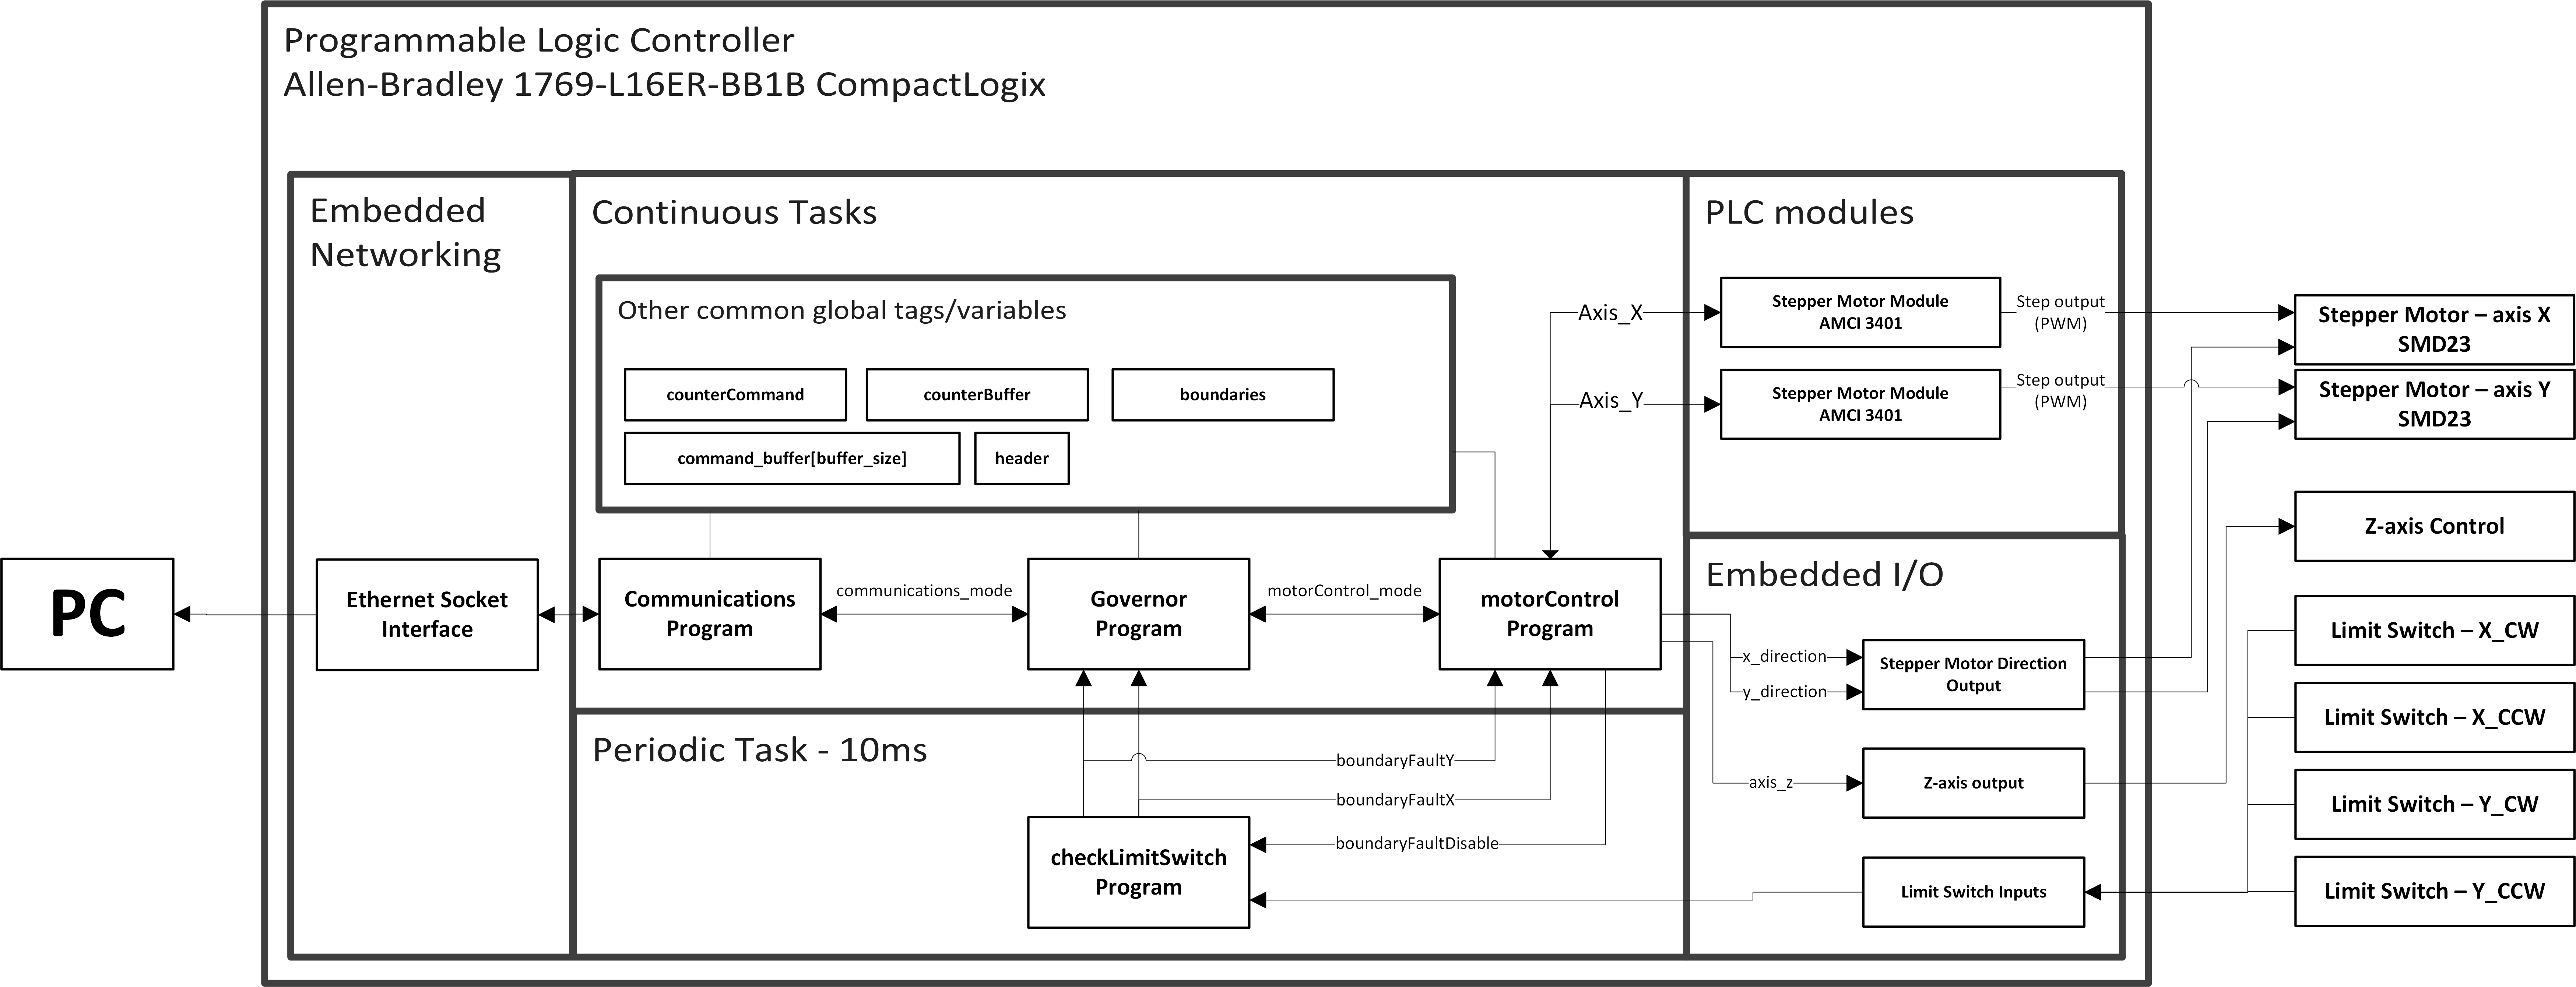
\includegraphics[width=\hsize]{figures/cncMachine/PLC_architecture}
		\captionof{figure}{The program and I/O architecture of the PLC. Arrows represent data flow, and when labelled, are global scope variables.}
		\label{fig:PLCarchitecture}
		\vspace*{\fill}
\end{landscape}



	\subsection{Governor}
	
		\begin{figure}[h]
			\centering
			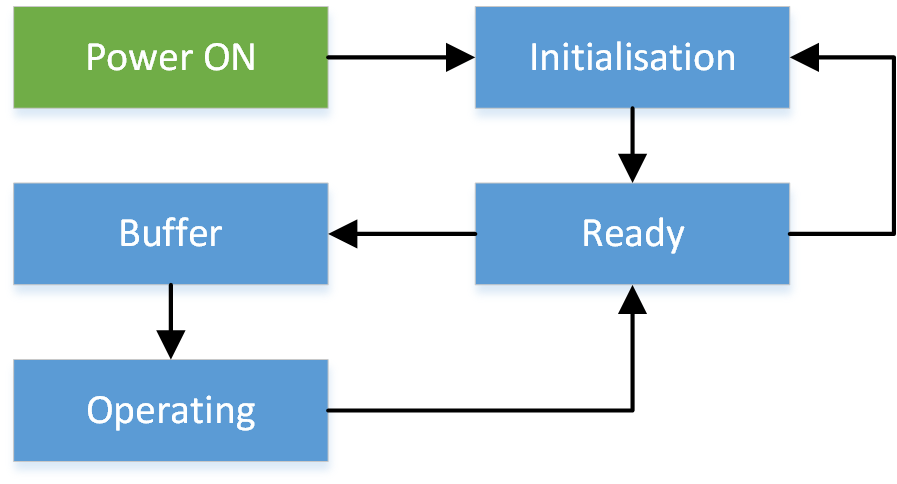
\includegraphics[width=0.5\textwidth]{figures/cncMachine/governor_simple.png}
			\caption{Governor States}
			\label{fig:governor-states}
		\end{figure}
		
		The Governor, shown in Figure ~\ref{fig:governor-states}, is a state machine that control the operation of the other programs in the DoodleBot system. The states are:
		
		\begin{description}
			\item[Power ON] DoodleBot waits for the user to press one of the Y limit switches to state A to start initialization.
			\item[Initialisation] The DoodleBot checks the boundaries and centres itself on a 'home' position. After this is complete it progresses to state B.
			\item[ready] The DoodleBot starts sending the 'ready' packet periodically to the PC, while waiting for a header to arrive. If a valid header arrives, it transitions to state C. If one of the Y limit switches are pressed, it returns to state A to run through the initialization routine once more.
			\item[Buffer] The DoodleBot begins requesting commands from the PC, filling the commandBuffer. When either the commandBuffer is full or all commands have been received, it progresses to state D.
			\item[Operating] The DoodleBot begins executing the commands in the commandBuffer. If there are still commands to received, it will continue to buffer when slots are freed up after being executed. After all commands have been processed the system returns to state B, ready for another header.
		\end{description}
		
		Please see Figure ~\ref{fig:PLC-flowcharts-governor} in Appendix ~\ref{ch:PLC-flowcharts} for more detailed information on how the Governor operates.

\subsection{Communications}
	
			\begin{figure}[h]
				\centering
				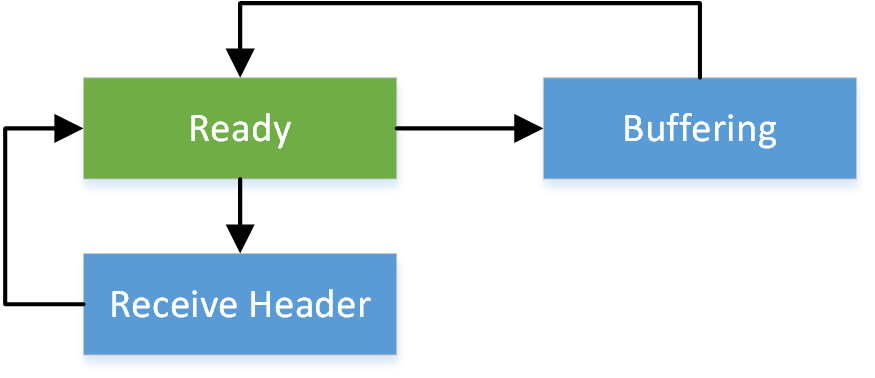
\includegraphics[width=0.5\textwidth]{figures/cncMachine/communications_simple.png}
				\caption{Communications States}
				\label{fig:comms-states}
			\end{figure}
	
	The Communications program, shown in Figure ~\ref{fig:comms-states}, has the role of communicating with the PC to populate the command buffer with the output of the PCs optimization stage. 

	
			\begin{description}
				\item[Ready] The Communications program does nothing.
				\item[Receive Header] The Communications program initializes the Ethernet socket interface and then starts requesting a header. If no header is received it continues to request until a valid one is received, in which case it returns to the Ready state and tells the Governor it is done.
				\item[Buffering] In the Buffer state, the Communications module requests commands and populating the command buffer, ensuring it doesn't overwrite data that hasn't been executed by motorControl yet. Once it has received the amount of commands specified in the header, it returns to the Ready state and informs the Governor it's done.
			\end{description}
			
		Please see Figure ~\ref{fig:communicationsStates} in Appendix ~\ref{ch:PLC-flowcharts} for more detailed information on how Communications operates.


\subsection{motorControl}

			\begin{figure}[h]
				\centering
				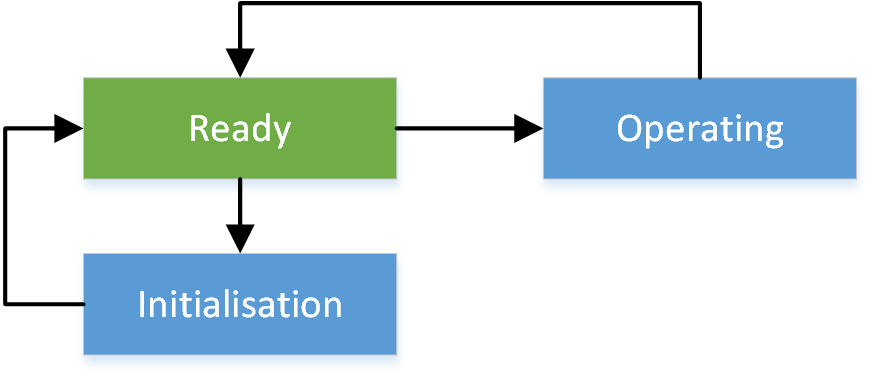
\includegraphics[width=0.5\textwidth]{figures/cncMachine/motorControl_simple.png}
				\caption{motorControl States}
				\label{fig:motorcontrol-states}
			\end{figure}
	
	The motorControl program, shown in Figure ~\ref{fig:motorcontrol-states}, has the role of controlling the electromechanical hardware via the AMCI 3401 module and the PLC Embedded I/O. 
	
			\begin{description}
				\item[Ready] The motorControl program does nothing.
				\item[Initialisation] The motorControl program runs its initialisation routine, which involves configuring the AMCI 3401 stepper motor modules and then running both motors in both directions until the limit switches are activated. This locates the boundaries of the CNC machine respective to the existing state of the motors, and allows the program to locate a centre point and set that to be the (0,0) point. It then returns to the Ready state and informs the Governor it's done.
				\item[Operating] In the operating state, motorControl reads the commands in the buffer and executes them. 'Move' type commands involve moving to a required point at a fixed velocity while retracting the drawing head. 'Draw' type commands involve extended the drawing head and then running a sampled velocity profile at the rate set in the header file.
			\end{description}
			
		Please see Section ~\ref{sec:PLC-flowcharts-motor}in Appendix ~\ref{ch:PLC-flowcharts} for more detailed information on how motorControl and the AMCI 3401 module operate.

	\subsubsection{Stepper Motor Direction Management}	
	\label{sec:stepperdirectionmanagement}
			Empirical observation of the AMCI 3401 modules in operation showed a significant delay (in the order of 2-3 seconds) between distinct commands. This delay was also present when switching between the Manual Move Clockwise and the Manual Move Counterclockwise commands. In contrast, changing the programmed speed while in either manual move state had negligible delay.
			
			This behaviour was a significant issue since the optimized velocity profiles require both axes to track the commands within the period of sampling (in the order of 30-150ms) to follow the required path and as such a 2-3 second delay would prevent proper operation.
			
			To overcome this problem, the DoodleBot controls the direction output via the PLC embedded DC output pins 0 and 1. Direction control is hence done  through code in the motorControl program rather than allow the AMCI 3401 modules to handle the task. The modules will just be constantly run with 'clockwise' commands and assume they are never making the direction switch. 
			
			To continue using Absolute Moves, this also required extra code to keep track of the current position.
			
			Please see Appendix ~\ref{sec:PLC-flowcharts-pos} for more detail on how this part of the code works. A flowchart of this code can be found in Figure ~\ref{fig:Direction and Positional Tracking}.
			
	\subsubsection{Draw Mode Initialisation - Dummy Commands}
			Section ~\ref{stepperdirectionmanagement} identified a method to eliminate the effect of the Stepper Motor lag between distinct commands by always commanding the AMCI 3401 modules to run in the same direction and controlling the Direction separately. There was however, still the initial lag when starting a velocity profile.
			
			To overcome this every velocity profile is padded with some 'dummy' commands that have the machine travel back very slowly and forth at the sample rate  (in the order of single steps), which means there is no noticeably drawn content. The command lag will means only these 'dummy commands' are skipped and ensures that when the real commands are processed they aren't skipped.
			
			At a sampling time of 40ms, 25 'dummy commands' were required to eliminate the module skipping 'real' commands.

	\subsubsection{Overcoming AMCI 3401 Internal Timer Issues}
			After experiencing some issues during testing, a conjectured model of the AMCI 3401's internal workings was made: "A new programmed speed is received by the AMCI 3401 while in a clockwise movement state. The programmed speed is the frequency of step pulses to produce per second and this translates to a period in between pulses. The AMCI 3401 then sets a timer to 0 and counts one period before producing the first step."
			
			The important note of this model to effect is that the internal timer is reset on every new programmed speed received. This assumption was made due to the observed effect of programmed speeds below a certain threshold not causing any movement. The model would explain the issue since if the period of step output is greater than the sample period, the timer would never actually approach the time in which it generates its first step and would keep resetting back to 0 with every command.
			
			Thus if this model were correct, there would be a minimum programmed speed threshold for the stepper modules to be able to move at all equal to $Speed_{minimum} = 1000ms/Sample_{time}$. So at 40ms, the minimum speed threshold would be 25 steps/second.
			
			To alleviate this effect, the DoodleBot has code that sets any code below this threshold to be equal to the minimum speed (except where the axis is completely stationary). 
			
			Further testing confirmed significantly better results. There are theoretical inaccuracies caused by the fact any velocity information below the threshold is lost, however this is significantly outweighed by the significant improvements found by using this fix. 

\subsection{checkLimitSwitch}
	The checkLimitSwitch program is run in a Periodic Task of 10ms and monitors the four limit switches. Upon detecting a rising edge (ie, the machine has hit the end of its range of motion) it alerts the motorControl program. If the motorControl program is in Operating Mode, it'll trigger an emergency stop and halt all operation.
	
	Please see Section ~\ref{sec:PLC-flowcharts-limit} in Appendix ~\ref{ch:PLC-flowcharts} for more detail on how checkLimitSwitch operates.